% !TEX TS-program = pdflatex
% !TEX root = ../tesi.tex

%************************************************
\chapter{Implementazione}
\label{chp:Implementazione}
%************************************************

In questo capitolo sarà presente l’analisi degli algoritmi che compongono il sistema riverberante creato. Gli algoritmi sono stati scritti nel linguaggio Faust sulla base delle ricerche svolte da Schroeder e Moorer e presentano le dovute modifiche che rispecchiano l’idea iniziale, vale a dire utilizzando parametri quali temperatura, pressione e tipologia del gas per variare la risposta del riverbero.

\section{Algoritmi di Schroeder}

I primi algoritmi sono stati creati partendo dalle soluzioni ottenute da Schroeder e utilizzati a scopo di test. L’obiettivo è stato quello di ricreare passo dopo passo le unità descritte nell’articolo Natural Sounding Artificial Reverberation. 

\subsection{Algoritmi fondamentali}

Partendo quindi dagli elementi fondamentali, abbiamo, come primo sistema il filtro Comb descritto in \ref{fig:dfl}.
\begin{code}
dfld(t, g) = ( + : de.delay(ma.SR,t-1))~(*(g)) : mem; //delay feed loop 
process = os.impulse : dfld(1000,.707);
\end{code}

Il codice presenta le variabili t e g che rappresentano rispettivamente il numero di campioni di ditardo e il moltiplicatore del feedback.
La funzione de.delay è utilizzata per il ritardo di un determinato numero di campioni.
Il simbolo \verb!~! permette l'utilizzo di una recursione, ovvero divide il segnale inviando una sua copia all'entrata del processo, creando \emph{feedback}
Il diagramma di questo codice è in figura \ref{fig:dflfaust}.

\bigskip

\begin{figure}[htp]
\centering
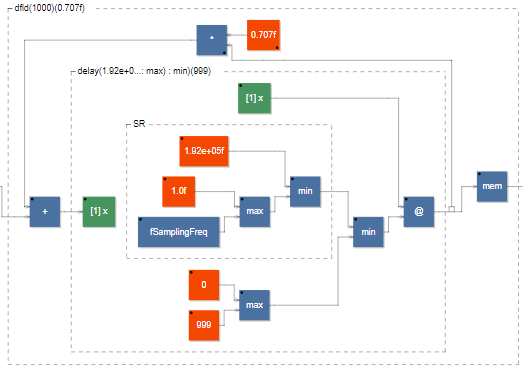
\includegraphics[width=%
0.80\textwidth]{dflfaust}
\caption{delay feedback loop}
\label{fig:dflfaust}
\end{figure}

Il secondo algoritmo derivato permette di realizzare un filtro All Pass, come quello descritto in figura \ref{fig:apf}

\begin{code}
apf(t,g) = _ <: *(-g) + (dfld(t,g)*(1-g^2));
process = os.impulse : apf(1,.71);
\end{code}

Il comportamento All Pass è dato dalla somma del segnale ritardato moltiplicato per $(1-g^2)$ e il segnale diretto moltiplicato per $-g$
Il diagramma di questo codice è in figura \ref{fig:apfaust}.

\begin{figure}[htp]
\centering
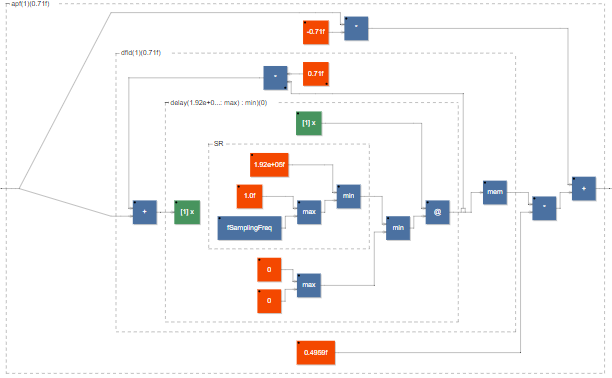
\includegraphics[width=%
0.90\textwidth]{apfaust}
\caption{All Pass}
\label{fig:apfaust}
\end{figure}

\subsection{Algoritmi derivati}

I prossimi algoritmi sono i successivi descritti da Schroeder. Presentano una serie di miglioramenti che auspicano ad una maggior naturalezza nella risposta del filtro. 
Come abbiamo visto in figura \ref{fig:apfmix}, creiamo un All Pass contenente un secondo All Pass e un delay al suo interno, per simulare il ritardo che intercorre tra il suono diretto e il suono riverberato.

\smallskip

il nuovo All Pass è dunque:
\begin{code}
dflda(t,g) =  (+ : de.delay(ma.SR,t-1) : apf(t,g))~ *(g) : mem;
\end{code}

Il suo diagramma lo troviamo in figura \ref{fig:dfldafaust}

\begin{figure}[htp]
\centering
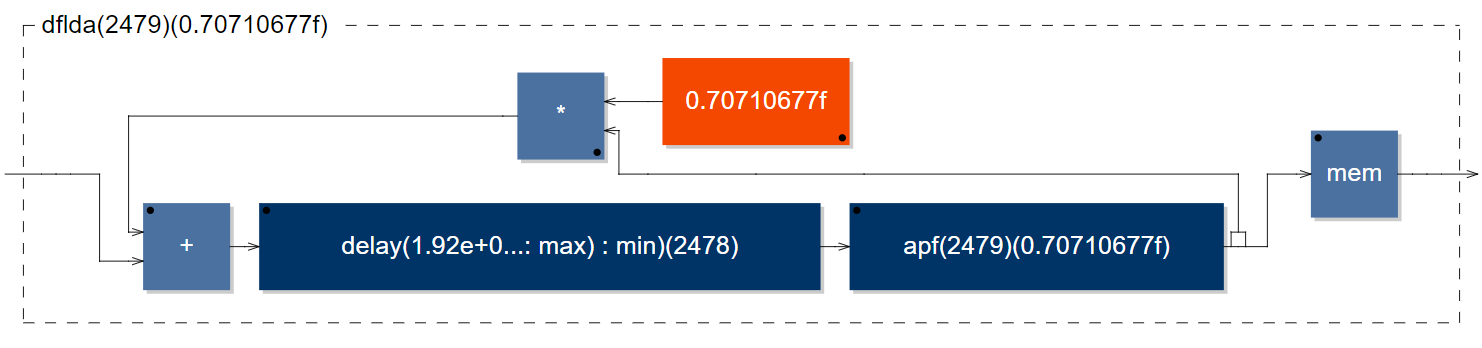
\includegraphics[width=%
0.90\textwidth]{dfldafaust}
\caption{Nuovo All Pass}
\label{fig:dfldafaust}
\end{figure}

Dato che abbiamo la necessità di missare il risultato del precedente filtro con il segnale diretto, creiamo un secondo ogetto che ci permette di farlo.

\begin{code}
apfn(t,g) = _ <: *(-g) + dflda(t,g) * (1-g^2);
\end{code}

\begin{figure}[htp]
\centering
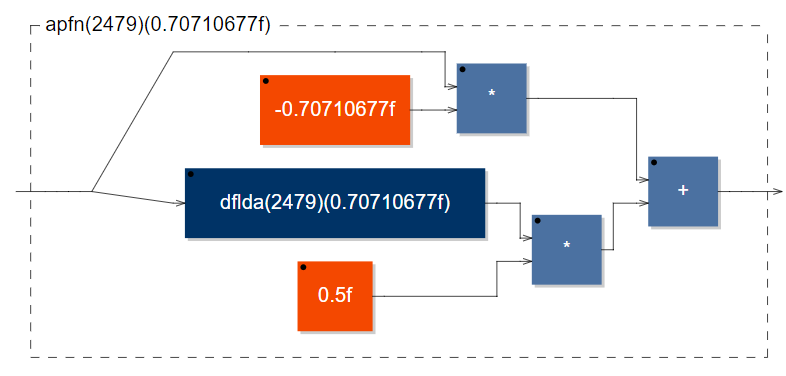
\includegraphics[width=%
0.70\textwidth]{apfmixfaust}
\caption{Nuovo All Pass con mix segnale diretto}
\label{fig:apfmixfaust}
\end{figure}

Il valore di g, inoltre, permette di decidere la quantità di segnale riverberato che vogliamo, come se fosse un pomello `'Dry/Wet''.

\subsection{Algoritmi Combinati}
Come già visto nel Capitolo 3, queste unità riverberanti non risultano particolaremente efficenti dal punto di vista della densità, se prese singolarmente, quindi il prossimo passo, come suggerito da Schroeder, è quello di crare delle reti di riverberatori combinando queste unità fondamentali.

\bigskip

Le due tipologie proposte consistono in una serie di All Pass connessi (figura \ref{fig:apfseq}), per la prima e, una serie di Comb connessi in cascata seguiti da 2 All Pass in serie, per la seconda.
Durante questa fase sono stati utilizzati numeri primi come valori dei ritardi in modo da evitare errori dovuti al campionamento.

L'algoritmo per la configurazione in serie risulta essere

\begin{code}
apfseq =  seq(i, 5, apf(ba.take(i+1, primet10),.7));
\end{code}

La lista ''primet10'' è stata caricata con i valori dei vari t. Come suggerito dall'autore, si è cercato di utilizzare numeri primi che mantenessero una relazione di $1/3$ l'uno dall'altro.
Il diagramma risultante è in figura \ref{fig:apfseqfaust}.

\begin{figure}[htp]
\centering
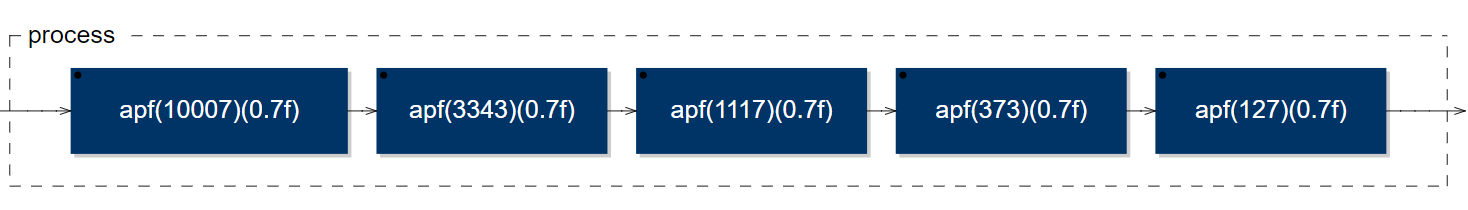
\includegraphics[width=%
0.90\textwidth]{apfseqfaust}
\caption{Sequenza di All Pass}
\label{fig:apfseqfaust}
\end{figure}

Il secondo algoritmo, per la configurazione `'Comb-All Pass'' vista in figura \ref{fig:comballpass}, è descritto nel seguente algoritmo

\begin{code}
reva((t,g,t1,g1),g2) = _<:_+(
    par(i,6, dflda(ba.take(i+1, t),G*ba.take(i+1,g))) :> 
    seq(i, 2, apfn(ba.take(4-i, t1),G*ba.take(i+1,g1))))*(g2);
process = _ : reva((primetc1,combg1,primetc2,combg2),G);
\end{code}

`'par'' e `'rev'' sono rispettivamente, composizione parallela e composizione sequenziale e ci permettono di creare una cascata di 6 Comb seguita da una sequenza di 2 All Pass. 

Il risultato è in figura \ref{fig:comballpassfaust}.

\begin{figure}[htp]
\centering
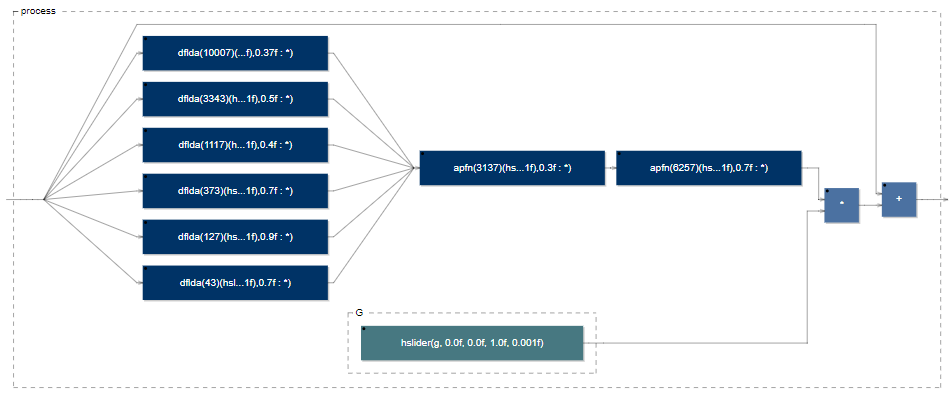
\includegraphics[width=%
1.2\textwidth]{comballpassfaust}
\caption{Algoritmo Comb-All Pass}
\label{fig:comballpassfaust}
\end{figure}

Quest'algoritmo risulta essere il più efficente ad ora e permette la riproduzione di oltre 1000 echi al secondo, un buon risultato considerando le stime effettute da Schroeder, ma che non corrisponde ad una riverberazione realistica e gradevole.

\section{Algoritmi di Moorer}

In seguito alla fase di test, il passo successivo è stato quello di implementare gli algoritmi di Moorer, in quanto risultano più efficenti dei precedenti. 
In questa sezione verranno inoltre inseriti i parametri ambientali ed utilizzati come controllo delle caratteristiche del riverbero. Le formule utilizzate per il calclo dei parametri sono le medesime viste nel capitolo \ref{chp:Filtri} ma con le dovute approssimazioni.

\bigskip

Il codice seguente descrive il filtro All Pass secondo le indicazioni di Moorer (visto in figura \ref{fig:apfmoorer}) e come già detto, senellisce i calcoli riducendo il numero delle moltiplicazioni ad 1.

\begin{code}
apfm(t, g) = _<: ((+ : _*(g)),_<:_,!,_+_ : _, zm(t) : ro.cross(2))~(0 -_) : +
with{
    zm(t) = de.delay(ma.SR,t);
};
\end{code}

\bigskip

Il grafico risultante è in figura \ref{fig:apfmoorerfaust}

\begin{figure}[htp]
\centering
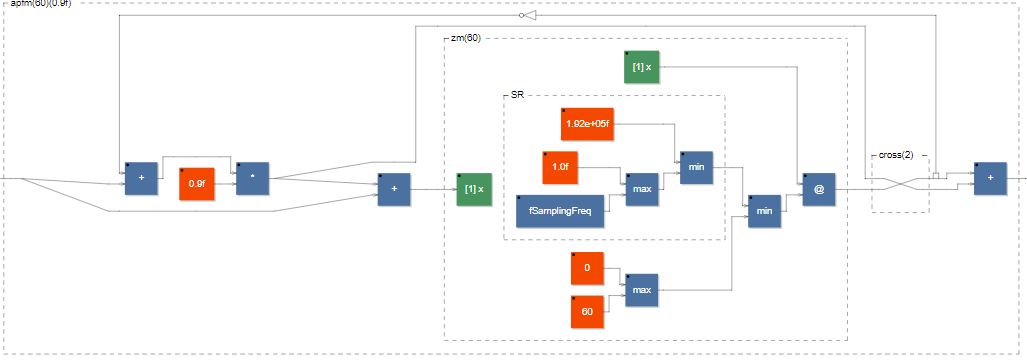
\includegraphics[width=%
1.2\textwidth]{apfmoorerfaust}
\caption{All Pass descritto da Moorer}
\label{fig:apfmoorerfaust}
\end{figure}
